% Graphic for TeX using PGF
% Title: /home/guillaume/Documents/umlclient.dia
% Creator: Dia v0.97.3
% CreationDate: Mon Feb 16 01:04:52 2015
% For: guillaume
% \usepackage{tikz}
% The following commands are not supported in PSTricks at present
% We define them conditionally, so when they are implemented,
% this pgf file will use them.
\ifx\du\undefined
  \newlength{\du}
\fi
\setlength{\du}{15\unitlength}

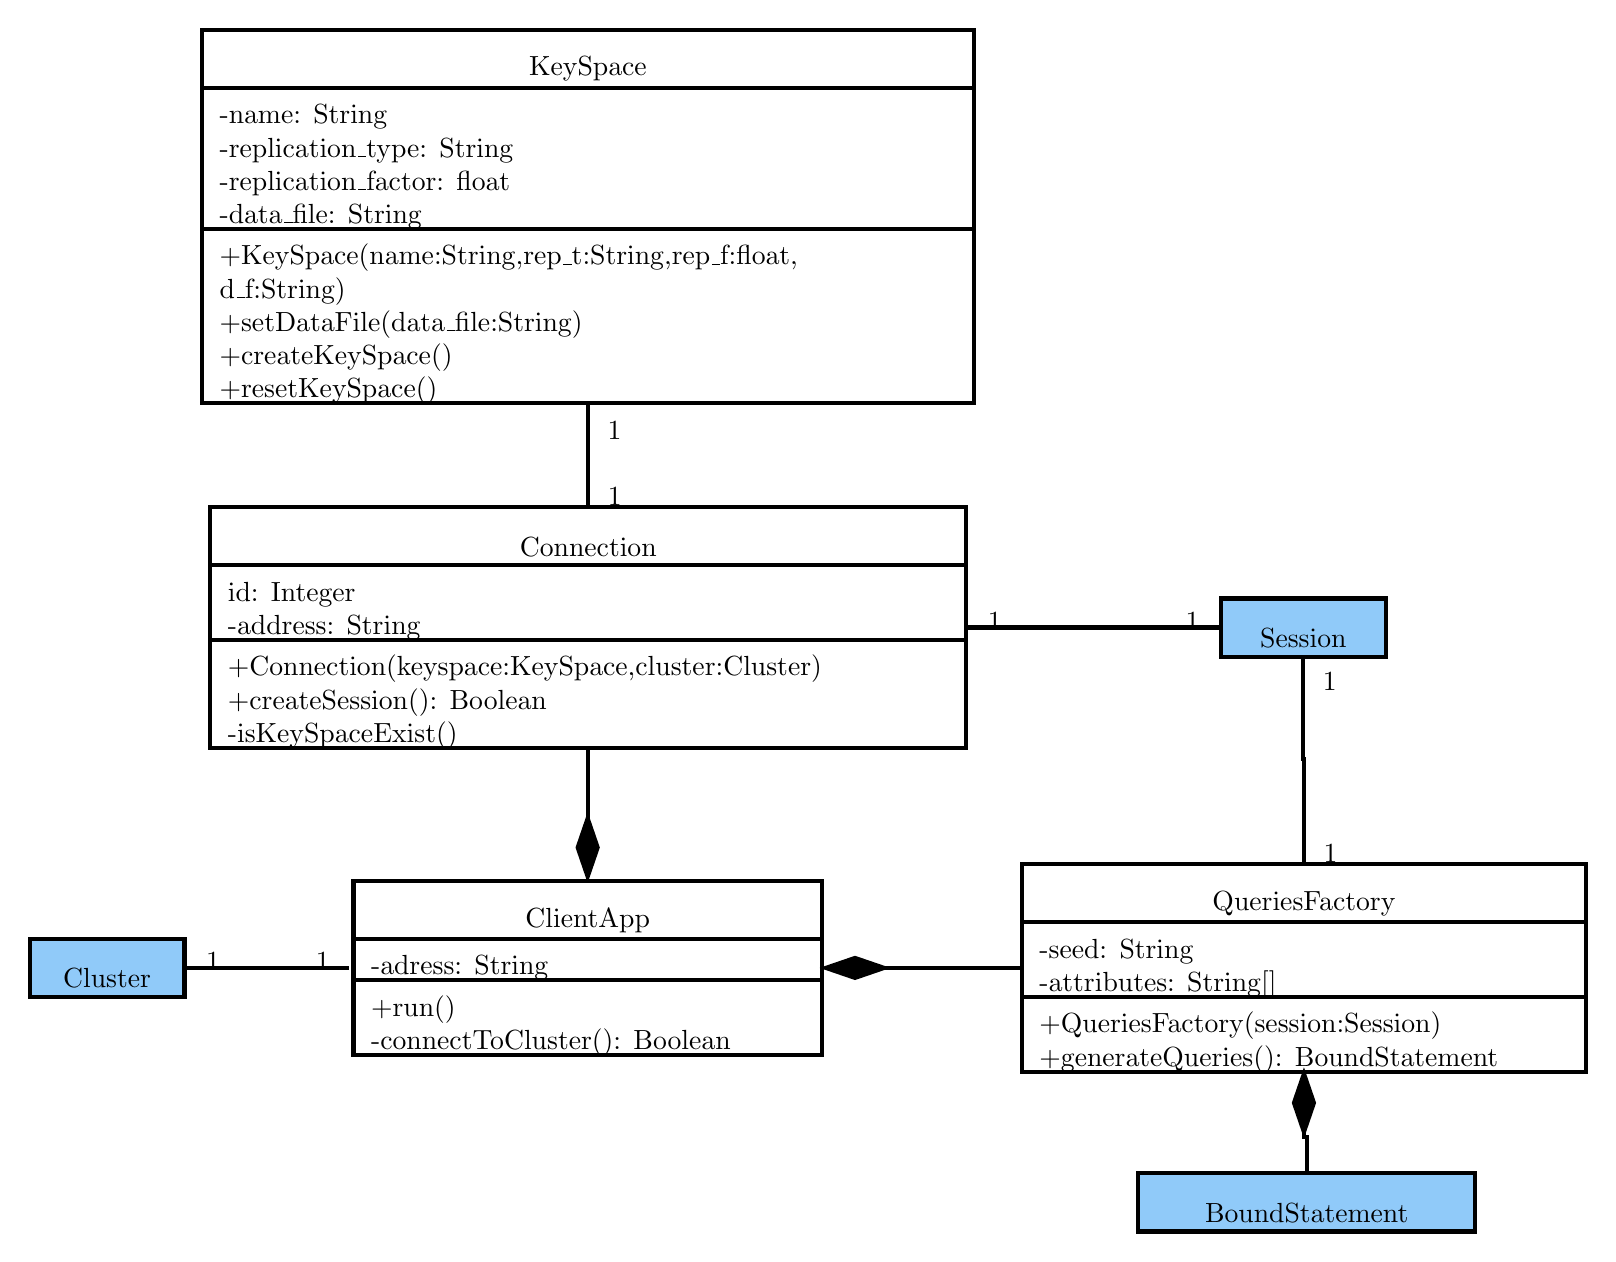
\begin{tikzpicture}
\pgftransformxscale{1.000000}
\pgftransformyscale{-1.000000}
\definecolor{dialinecolor}{rgb}{0.000000, 0.000000, 0.000000}
\pgfsetstrokecolor{dialinecolor}
\definecolor{dialinecolor}{rgb}{1.000000, 1.000000, 1.000000}
\pgfsetfillcolor{dialinecolor}
\pgfsetlinewidth{0.100000\du}
\pgfsetdash{}{0pt}
\definecolor{dialinecolor}{rgb}{1.000000, 1.000000, 1.000000}
\pgfsetfillcolor{dialinecolor}
\fill (28.250000\du,24.500000\du)--(28.250000\du,25.900000\du)--(39.530000\du,25.900000\du)--(39.530000\du,24.500000\du)--cycle;
\definecolor{dialinecolor}{rgb}{0.000000, 0.000000, 0.000000}
\pgfsetstrokecolor{dialinecolor}
\draw (28.250000\du,24.500000\du)--(28.250000\du,25.900000\du)--(39.530000\du,25.900000\du)--(39.530000\du,24.500000\du)--cycle;
% setfont left to latex
\definecolor{dialinecolor}{rgb}{0.000000, 0.000000, 0.000000}
\pgfsetstrokecolor{dialinecolor}
\node at (33.890000\du,25.450000\du){ClientApp};
\definecolor{dialinecolor}{rgb}{1.000000, 1.000000, 1.000000}
\pgfsetfillcolor{dialinecolor}
\fill (28.250000\du,25.900000\du)--(28.250000\du,26.900000\du)--(39.530000\du,26.900000\du)--(39.530000\du,25.900000\du)--cycle;
\definecolor{dialinecolor}{rgb}{0.000000, 0.000000, 0.000000}
\pgfsetstrokecolor{dialinecolor}
\draw (28.250000\du,25.900000\du)--(28.250000\du,26.900000\du)--(39.530000\du,26.900000\du)--(39.530000\du,25.900000\du)--cycle;
% setfont left to latex
\definecolor{dialinecolor}{rgb}{0.000000, 0.000000, 0.000000}
\pgfsetstrokecolor{dialinecolor}
\node[anchor=west] at (28.400000\du,26.600000\du){-adress: String};
\definecolor{dialinecolor}{rgb}{1.000000, 1.000000, 1.000000}
\pgfsetfillcolor{dialinecolor}
\fill (28.250000\du,26.900000\du)--(28.250000\du,28.700000\du)--(39.530000\du,28.700000\du)--(39.530000\du,26.900000\du)--cycle;
\definecolor{dialinecolor}{rgb}{0.000000, 0.000000, 0.000000}
\pgfsetstrokecolor{dialinecolor}
\draw (28.250000\du,26.900000\du)--(28.250000\du,28.700000\du)--(39.530000\du,28.700000\du)--(39.530000\du,26.900000\du)--cycle;
% setfont left to latex
\definecolor{dialinecolor}{rgb}{0.000000, 0.000000, 0.000000}
\pgfsetstrokecolor{dialinecolor}
\node[anchor=west] at (28.400000\du,27.600000\du){+run()};
% setfont left to latex
\definecolor{dialinecolor}{rgb}{0.000000, 0.000000, 0.000000}
\pgfsetstrokecolor{dialinecolor}
\node[anchor=west] at (28.400000\du,28.400000\du){-connectToCluster(): Boolean};
\pgfsetlinewidth{0.100000\du}
\pgfsetdash{}{0pt}
\definecolor{dialinecolor}{rgb}{0.564706, 0.792157, 0.976471}
\pgfsetfillcolor{dialinecolor}
\fill (49.150000\du,17.700000\du)--(49.150000\du,19.100000\du)--(53.112500\du,19.100000\du)--(53.112500\du,17.700000\du)--cycle;
\definecolor{dialinecolor}{rgb}{0.000000, 0.000000, 0.000000}
\pgfsetstrokecolor{dialinecolor}
\draw (49.150000\du,17.700000\du)--(49.150000\du,19.100000\du)--(53.112500\du,19.100000\du)--(53.112500\du,17.700000\du)--cycle;
% setfont left to latex
\definecolor{dialinecolor}{rgb}{0.000000, 0.000000, 0.000000}
\pgfsetstrokecolor{dialinecolor}
\node at (51.131250\du,18.650000\du){Session};
\pgfsetlinewidth{0.100000\du}
\pgfsetdash{}{0pt}
\definecolor{dialinecolor}{rgb}{0.564706, 0.792157, 0.976471}
\pgfsetfillcolor{dialinecolor}
\fill (20.450000\du,25.900000\du)--(20.450000\du,27.300000\du)--(24.177500\du,27.300000\du)--(24.177500\du,25.900000\du)--cycle;
\definecolor{dialinecolor}{rgb}{0.000000, 0.000000, 0.000000}
\pgfsetstrokecolor{dialinecolor}
\draw (20.450000\du,25.900000\du)--(20.450000\du,27.300000\du)--(24.177500\du,27.300000\du)--(24.177500\du,25.900000\du)--cycle;
% setfont left to latex
\definecolor{dialinecolor}{rgb}{0.000000, 0.000000, 0.000000}
\pgfsetstrokecolor{dialinecolor}
\node at (22.313750\du,26.850000\du){Cluster};
\pgfsetlinewidth{0.100000\du}
\pgfsetdash{}{0pt}
\definecolor{dialinecolor}{rgb}{1.000000, 1.000000, 1.000000}
\pgfsetfillcolor{dialinecolor}
\fill (44.350000\du,24.100000\du)--(44.350000\du,25.500000\du)--(57.940000\du,25.500000\du)--(57.940000\du,24.100000\du)--cycle;
\definecolor{dialinecolor}{rgb}{0.000000, 0.000000, 0.000000}
\pgfsetstrokecolor{dialinecolor}
\draw (44.350000\du,24.100000\du)--(44.350000\du,25.500000\du)--(57.940000\du,25.500000\du)--(57.940000\du,24.100000\du)--cycle;
% setfont left to latex
\definecolor{dialinecolor}{rgb}{0.000000, 0.000000, 0.000000}
\pgfsetstrokecolor{dialinecolor}
\node at (51.145000\du,25.050000\du){QueriesFactory};
\definecolor{dialinecolor}{rgb}{1.000000, 1.000000, 1.000000}
\pgfsetfillcolor{dialinecolor}
\fill (44.350000\du,25.500000\du)--(44.350000\du,27.300000\du)--(57.940000\du,27.300000\du)--(57.940000\du,25.500000\du)--cycle;
\definecolor{dialinecolor}{rgb}{0.000000, 0.000000, 0.000000}
\pgfsetstrokecolor{dialinecolor}
\draw (44.350000\du,25.500000\du)--(44.350000\du,27.300000\du)--(57.940000\du,27.300000\du)--(57.940000\du,25.500000\du)--cycle;
% setfont left to latex
\definecolor{dialinecolor}{rgb}{0.000000, 0.000000, 0.000000}
\pgfsetstrokecolor{dialinecolor}
\node[anchor=west] at (44.500000\du,26.200000\du){-seed: String};
% setfont left to latex
\definecolor{dialinecolor}{rgb}{0.000000, 0.000000, 0.000000}
\pgfsetstrokecolor{dialinecolor}
\node[anchor=west] at (44.500000\du,27.000000\du){-attributes: String\ensuremath{[}\ensuremath{]}};
\definecolor{dialinecolor}{rgb}{1.000000, 1.000000, 1.000000}
\pgfsetfillcolor{dialinecolor}
\fill (44.350000\du,27.300000\du)--(44.350000\du,29.100000\du)--(57.940000\du,29.100000\du)--(57.940000\du,27.300000\du)--cycle;
\definecolor{dialinecolor}{rgb}{0.000000, 0.000000, 0.000000}
\pgfsetstrokecolor{dialinecolor}
\draw (44.350000\du,27.300000\du)--(44.350000\du,29.100000\du)--(57.940000\du,29.100000\du)--(57.940000\du,27.300000\du)--cycle;
% setfont left to latex
\definecolor{dialinecolor}{rgb}{0.000000, 0.000000, 0.000000}
\pgfsetstrokecolor{dialinecolor}
\node[anchor=west] at (44.500000\du,28.000000\du){+QueriesFactory(session:Session)};
% setfont left to latex
\definecolor{dialinecolor}{rgb}{0.000000, 0.000000, 0.000000}
\pgfsetstrokecolor{dialinecolor}
\node[anchor=west] at (44.500000\du,28.800000\du){+generateQueries(): BoundStatement};
\pgfsetlinewidth{0.100000\du}
\pgfsetdash{}{0pt}
\definecolor{dialinecolor}{rgb}{1.000000, 1.000000, 1.000000}
\pgfsetfillcolor{dialinecolor}
\fill (24.600000\du,4.000000\du)--(24.600000\du,5.400000\du)--(43.195000\du,5.400000\du)--(43.195000\du,4.000000\du)--cycle;
\definecolor{dialinecolor}{rgb}{0.000000, 0.000000, 0.000000}
\pgfsetstrokecolor{dialinecolor}
\draw (24.600000\du,4.000000\du)--(24.600000\du,5.400000\du)--(43.195000\du,5.400000\du)--(43.195000\du,4.000000\du)--cycle;
% setfont left to latex
\definecolor{dialinecolor}{rgb}{0.000000, 0.000000, 0.000000}
\pgfsetstrokecolor{dialinecolor}
\node at (33.897500\du,4.950000\du){KeySpace};
\definecolor{dialinecolor}{rgb}{1.000000, 1.000000, 1.000000}
\pgfsetfillcolor{dialinecolor}
\fill (24.600000\du,5.400000\du)--(24.600000\du,8.800000\du)--(43.195000\du,8.800000\du)--(43.195000\du,5.400000\du)--cycle;
\definecolor{dialinecolor}{rgb}{0.000000, 0.000000, 0.000000}
\pgfsetstrokecolor{dialinecolor}
\draw (24.600000\du,5.400000\du)--(24.600000\du,8.800000\du)--(43.195000\du,8.800000\du)--(43.195000\du,5.400000\du)--cycle;
% setfont left to latex
\definecolor{dialinecolor}{rgb}{0.000000, 0.000000, 0.000000}
\pgfsetstrokecolor{dialinecolor}
\node[anchor=west] at (24.750000\du,6.100000\du){-name: String};
% setfont left to latex
\definecolor{dialinecolor}{rgb}{0.000000, 0.000000, 0.000000}
\pgfsetstrokecolor{dialinecolor}
\node[anchor=west] at (24.750000\du,6.900000\du){-replication\_type: String};
% setfont left to latex
\definecolor{dialinecolor}{rgb}{0.000000, 0.000000, 0.000000}
\pgfsetstrokecolor{dialinecolor}
\node[anchor=west] at (24.750000\du,7.700000\du){-replication\_factor: float};
% setfont left to latex
\definecolor{dialinecolor}{rgb}{0.000000, 0.000000, 0.000000}
\pgfsetstrokecolor{dialinecolor}
\node[anchor=west] at (24.750000\du,8.500000\du){-data\_file: String};
\definecolor{dialinecolor}{rgb}{1.000000, 1.000000, 1.000000}
\pgfsetfillcolor{dialinecolor}
\fill (24.600000\du,8.800000\du)--(24.600000\du,13.000000\du)--(43.195000\du,13.000000\du)--(43.195000\du,8.800000\du)--cycle;
\definecolor{dialinecolor}{rgb}{0.000000, 0.000000, 0.000000}
\pgfsetstrokecolor{dialinecolor}
\draw (24.600000\du,8.800000\du)--(24.600000\du,13.000000\du)--(43.195000\du,13.000000\du)--(43.195000\du,8.800000\du)--cycle;
% setfont left to latex
\definecolor{dialinecolor}{rgb}{0.000000, 0.000000, 0.000000}
\pgfsetstrokecolor{dialinecolor}
\node[anchor=west] at (24.750000\du,9.500000\du){+KeySpace(name:String,rep\_t:String,rep\_f:float,};
\definecolor{dialinecolor}{rgb}{0.000000, 0.000000, 0.000000}
\pgfsetstrokecolor{dialinecolor}
\node[anchor=west] at (24.750000\du,10.300000\du){          d\_f:String)};
% setfont left to latex
\definecolor{dialinecolor}{rgb}{0.000000, 0.000000, 0.000000}
\pgfsetstrokecolor{dialinecolor}
\node[anchor=west] at (24.750000\du,11.100000\du){+setDataFile(data\_file:String)};
% setfont left to latex
\definecolor{dialinecolor}{rgb}{0.000000, 0.000000, 0.000000}
\pgfsetstrokecolor{dialinecolor}
\node[anchor=west] at (24.750000\du,11.900000\du){+createKeySpace()};
% setfont left to latex
\definecolor{dialinecolor}{rgb}{0.000000, 0.000000, 0.000000}
\pgfsetstrokecolor{dialinecolor}
\node[anchor=west] at (24.750000\du,12.700000\du){+resetKeySpace()};
\pgfsetlinewidth{0.100000\du}
\pgfsetdash{}{0pt}
\definecolor{dialinecolor}{rgb}{0.564706, 0.792157, 0.976471}
\pgfsetfillcolor{dialinecolor}
\fill (47.150000\du,31.550000\du)--(47.150000\du,32.950000\du)--(55.272500\du,32.950000\du)--(55.272500\du,31.550000\du)--cycle;
\definecolor{dialinecolor}{rgb}{0.000000, 0.000000, 0.000000}
\pgfsetstrokecolor{dialinecolor}
\draw (47.150000\du,31.550000\du)--(47.150000\du,32.950000\du)--(55.272500\du,32.950000\du)--(55.272500\du,31.550000\du)--cycle;
% setfont left to latex
\definecolor{dialinecolor}{rgb}{0.000000, 0.000000, 0.000000}
\pgfsetstrokecolor{dialinecolor}
\node at (51.211250\du,32.500000\du){BoundStatement};
\pgfsetlinewidth{0.100000\du}
\pgfsetdash{}{0pt}
\definecolor{dialinecolor}{rgb}{1.000000, 1.000000, 1.000000}
\pgfsetfillcolor{dialinecolor}
\fill (24.800000\du,15.500000\du)--(24.800000\du,16.900000\du)--(43.010000\du,16.900000\du)--(43.010000\du,15.500000\du)--cycle;
\definecolor{dialinecolor}{rgb}{0.000000, 0.000000, 0.000000}
\pgfsetstrokecolor{dialinecolor}
\draw (24.800000\du,15.500000\du)--(24.800000\du,16.900000\du)--(43.010000\du,16.900000\du)--(43.010000\du,15.500000\du)--cycle;
% setfont left to latex
\definecolor{dialinecolor}{rgb}{0.000000, 0.000000, 0.000000}
\pgfsetstrokecolor{dialinecolor}
\node at (33.905000\du,16.450000\du){Connection};
\definecolor{dialinecolor}{rgb}{1.000000, 1.000000, 1.000000}
\pgfsetfillcolor{dialinecolor}
\fill (24.800000\du,16.900000\du)--(24.800000\du,18.700000\du)--(43.010000\du,18.700000\du)--(43.010000\du,16.900000\du)--cycle;
\definecolor{dialinecolor}{rgb}{0.000000, 0.000000, 0.000000}
\pgfsetstrokecolor{dialinecolor}
\draw (24.800000\du,16.900000\du)--(24.800000\du,18.700000\du)--(43.010000\du,18.700000\du)--(43.010000\du,16.900000\du)--cycle;
% setfont left to latex
\definecolor{dialinecolor}{rgb}{0.000000, 0.000000, 0.000000}
\pgfsetstrokecolor{dialinecolor}
\node[anchor=west] at (24.950000\du,17.600000\du){ id: Integer};
% setfont left to latex
\definecolor{dialinecolor}{rgb}{0.000000, 0.000000, 0.000000}
\pgfsetstrokecolor{dialinecolor}
\node[anchor=west] at (24.950000\du,18.400000\du){-address: String};
\definecolor{dialinecolor}{rgb}{1.000000, 1.000000, 1.000000}
\pgfsetfillcolor{dialinecolor}
\fill (24.800000\du,18.700000\du)--(24.800000\du,21.300000\du)--(43.010000\du,21.300000\du)--(43.010000\du,18.700000\du)--cycle;
\definecolor{dialinecolor}{rgb}{0.000000, 0.000000, 0.000000}
\pgfsetstrokecolor{dialinecolor}
\draw (24.800000\du,18.700000\du)--(24.800000\du,21.300000\du)--(43.010000\du,21.300000\du)--(43.010000\du,18.700000\du)--cycle;
% setfont left to latex
\definecolor{dialinecolor}{rgb}{0.000000, 0.000000, 0.000000}
\pgfsetstrokecolor{dialinecolor}
\node[anchor=west] at (24.950000\du,19.400000\du){+Connection(keyspace:KeySpace,cluster:Cluster)};
% setfont left to latex
\definecolor{dialinecolor}{rgb}{0.000000, 0.000000, 0.000000}
\pgfsetstrokecolor{dialinecolor}
\node[anchor=west] at (24.950000\du,20.200000\du){+createSession(): Boolean};
% setfont left to latex
\definecolor{dialinecolor}{rgb}{0.000000, 0.000000, 0.000000}
\pgfsetstrokecolor{dialinecolor}
\node[anchor=west] at (24.950000\du,21.000000\du){-isKeySpaceExist()};
\pgfsetlinewidth{0.100000\du}
\pgfsetdash{}{0pt}
\pgfsetmiterjoin
\pgfsetbuttcap
{
\definecolor{dialinecolor}{rgb}{0.000000, 0.000000, 0.000000}
\pgfsetfillcolor{dialinecolor}
% was here!!!
\definecolor{dialinecolor}{rgb}{0.000000, 0.000000, 0.000000}
\pgfsetstrokecolor{dialinecolor}
\draw (49.099504\du,18.400000\du)--(49.049504\du,18.400000\du)--(43.110279\du,18.400000\du)--(43.060279\du,18.400000\du);
}
% setfont left to latex
\definecolor{dialinecolor}{rgb}{0.000000, 0.000000, 0.000000}
\pgfsetstrokecolor{dialinecolor}
\node[anchor=east] at (48.899504\du,18.250000\du){1};
\definecolor{dialinecolor}{rgb}{0.000000, 0.000000, 0.000000}
\pgfsetstrokecolor{dialinecolor}
\node[anchor=west] at (43.260279\du,18.250000\du){1};
\pgfsetlinewidth{0.100000\du}
\pgfsetdash{}{0pt}
\pgfsetmiterjoin
\pgfsetbuttcap
{
\definecolor{dialinecolor}{rgb}{0.000000, 0.000000, 0.000000}
\pgfsetfillcolor{dialinecolor}
% was here!!!
\definecolor{dialinecolor}{rgb}{0.000000, 0.000000, 0.000000}
\pgfsetstrokecolor{dialinecolor}
\draw (33.897500\du,13.050278\du)--(33.897500\du,14.249959\du)--(33.905000\du,14.249959\du)--(33.905000\du,15.449640\du);
}
% setfont left to latex
\definecolor{dialinecolor}{rgb}{0.000000, 0.000000, 0.000000}
\pgfsetstrokecolor{dialinecolor}
\node[anchor=west] at (34.097500\du,13.650278\du){1};
\definecolor{dialinecolor}{rgb}{0.000000, 0.000000, 0.000000}
\pgfsetstrokecolor{dialinecolor}
\node[anchor=west] at (34.105000\du,15.249640\du){1};
\pgfsetlinewidth{0.100000\du}
\pgfsetdash{}{0pt}
\pgfsetmiterjoin
\pgfsetbuttcap
{
\definecolor{dialinecolor}{rgb}{0.000000, 0.000000, 0.000000}
\pgfsetfillcolor{dialinecolor}
% was here!!!
\definecolor{dialinecolor}{rgb}{0.000000, 0.000000, 0.000000}
\pgfsetstrokecolor{dialinecolor}
\draw (33.905000\du,21.350360\du)--(33.905000\du,22.525046\du)--(33.890000\du,22.525046\du)--(33.890000\du,24.399731\du);
}
\definecolor{dialinecolor}{rgb}{0.000000, 0.000000, 0.000000}
\pgfsetstrokecolor{dialinecolor}
\draw (33.905000\du,21.350360\du)--(33.905000\du,22.525046\du)--(33.890000\du,22.525046\du)--(33.890000\du,23.141153\du);
\pgfsetdash{}{0pt}
\pgfsetmiterjoin
\pgfsetbuttcap
\definecolor{dialinecolor}{rgb}{0.000000, 0.000000, 0.000000}
\pgfsetfillcolor{dialinecolor}
\fill (33.890000\du,24.399731\du)--(33.650000\du,23.699731\du)--(33.890000\du,22.999731\du)--(34.130000\du,23.699731\du)--cycle;
\pgfsetlinewidth{0.100000\du}
\pgfsetdash{}{0pt}
\pgfsetmiterjoin
\pgfsetbuttcap
\definecolor{dialinecolor}{rgb}{0.000000, 0.000000, 0.000000}
\pgfsetstrokecolor{dialinecolor}
\draw (33.890000\du,24.399731\du)--(33.650000\du,23.699731\du)--(33.890000\du,22.999731\du)--(34.130000\du,23.699731\du)--cycle;
% setfont left to latex
\pgfsetlinewidth{0.100000\du}
\pgfsetdash{}{0pt}
\pgfsetmiterjoin
\pgfsetbuttcap
{
\definecolor{dialinecolor}{rgb}{0.000000, 0.000000, 0.000000}
\pgfsetfillcolor{dialinecolor}
% was here!!!
\definecolor{dialinecolor}{rgb}{0.000000, 0.000000, 0.000000}
\pgfsetstrokecolor{dialinecolor}
\draw (44.299582\du,26.600000\du)--(44.249582\du,26.600000\du)--(40.380350\du,26.600000\du)--(39.630350\du,26.600000\du);
}
\definecolor{dialinecolor}{rgb}{0.000000, 0.000000, 0.000000}
\pgfsetstrokecolor{dialinecolor}
\draw (44.299582\du,26.600000\du)--(44.249582\du,26.600000\du)--(40.380350\du,26.600000\du)--(40.888929\du,26.600000\du);
\pgfsetdash{}{0pt}
\pgfsetmiterjoin
\pgfsetbuttcap
\definecolor{dialinecolor}{rgb}{0.000000, 0.000000, 0.000000}
\pgfsetfillcolor{dialinecolor}
\fill (39.630350\du,26.600000\du)--(40.330350\du,26.360000\du)--(41.030350\du,26.600000\du)--(40.330350\du,26.840000\du)--cycle;
\pgfsetlinewidth{0.100000\du}
\pgfsetdash{}{0pt}
\pgfsetmiterjoin
\pgfsetbuttcap
\definecolor{dialinecolor}{rgb}{0.000000, 0.000000, 0.000000}
\pgfsetstrokecolor{dialinecolor}
\draw (39.630350\du,26.600000\du)--(40.330350\du,26.360000\du)--(41.030350\du,26.600000\du)--(40.330350\du,26.840000\du)--cycle;
% setfont left to latex
\pgfsetlinewidth{0.100000\du}
\pgfsetdash{}{0pt}
\pgfsetmiterjoin
\pgfsetbuttcap
{
\definecolor{dialinecolor}{rgb}{0.000000, 0.000000, 0.000000}
\pgfsetfillcolor{dialinecolor}
% was here!!!
\definecolor{dialinecolor}{rgb}{0.000000, 0.000000, 0.000000}
\pgfsetstrokecolor{dialinecolor}
\draw (51.211250\du,31.499634\du)--(51.211250\du,30.674973\du)--(51.145000\du,30.674973\du)--(51.145000\du,29.150311\du);
}
\definecolor{dialinecolor}{rgb}{0.000000, 0.000000, 0.000000}
\pgfsetstrokecolor{dialinecolor}
\draw (51.211250\du,31.499634\du)--(51.211250\du,30.674973\du)--(51.145000\du,30.674973\du)--(51.145000\du,30.408890\du);
\pgfsetdash{}{0pt}
\pgfsetmiterjoin
\pgfsetbuttcap
\definecolor{dialinecolor}{rgb}{0.000000, 0.000000, 0.000000}
\pgfsetfillcolor{dialinecolor}
\fill (51.145000\du,29.150311\du)--(51.385000\du,29.850311\du)--(51.145000\du,30.550311\du)--(50.905000\du,29.850311\du)--cycle;
\pgfsetlinewidth{0.100000\du}
\pgfsetdash{}{0pt}
\pgfsetmiterjoin
\pgfsetbuttcap
\definecolor{dialinecolor}{rgb}{0.000000, 0.000000, 0.000000}
\pgfsetstrokecolor{dialinecolor}
\draw (51.145000\du,29.150311\du)--(51.385000\du,29.850311\du)--(51.145000\du,30.550311\du)--(50.905000\du,29.850311\du)--cycle;
% setfont left to latex
\pgfsetlinewidth{0.100000\du}
\pgfsetdash{}{0pt}
\pgfsetmiterjoin
\pgfsetbuttcap
{
\definecolor{dialinecolor}{rgb}{0.000000, 0.000000, 0.000000}
\pgfsetfillcolor{dialinecolor}
% was here!!!
\definecolor{dialinecolor}{rgb}{0.000000, 0.000000, 0.000000}
\pgfsetstrokecolor{dialinecolor}
\draw (24.227880\du,26.600000\du)--(24.738828\du,26.600000\du)--(24.738828\du,26.600000\du)--(28.149851\du,26.600000\du);
}
% setfont left to latex
\definecolor{dialinecolor}{rgb}{0.000000, 0.000000, 0.000000}
\pgfsetstrokecolor{dialinecolor}
\node[anchor=west] at (24.427880\du,26.450000\du){1};
\definecolor{dialinecolor}{rgb}{0.000000, 0.000000, 0.000000}
\pgfsetstrokecolor{dialinecolor}
\node[anchor=east] at (27.949851\du,26.450000\du){1};
\pgfsetlinewidth{0.100000\du}
\pgfsetdash{}{0pt}
\pgfsetmiterjoin
\pgfsetbuttcap
{
\definecolor{dialinecolor}{rgb}{0.000000, 0.000000, 0.000000}
\pgfsetfillcolor{dialinecolor}
% was here!!!
\definecolor{dialinecolor}{rgb}{0.000000, 0.000000, 0.000000}
\pgfsetstrokecolor{dialinecolor}
\draw (51.131250\du,19.100000\du)--(51.131250\du,21.574844\du)--(51.145000\du,21.574844\du)--(51.145000\du,24.049689\du);
}
% setfont left to latex
\definecolor{dialinecolor}{rgb}{0.000000, 0.000000, 0.000000}
\pgfsetstrokecolor{dialinecolor}
\node[anchor=west] at (51.331250\du,19.700000\du){1};
\definecolor{dialinecolor}{rgb}{0.000000, 0.000000, 0.000000}
\pgfsetstrokecolor{dialinecolor}
\node[anchor=west] at (51.345000\du,23.849689\du){1};
\end{tikzpicture}
